\section{Introduction}
\subsection{}
\setbeamertemplate{footline}[frame number]
\begin{frame}
\frametitle{Motivation}
\vspace{-0.2 cm}
\textcolor{red}{\textbf{Study a simplified mathematical model for the storage of radioactive waste}}
\\
\vspace{0.2 cm}
\textcolor{cadmiumgreen}{\textbf{Potential serious environmental hazard. Need for accurate simulation.}}
\\
\vspace*{0.2 cm}
\textcolor{cadmiumgreen}{\textbf{Quantify the error, propose robust algorithms, and save computational time.}}
\invisible<1>{
\begin{minipage}{0.6 \linewidth}
\vspace*{-1.9 cm}
\begin{equation*}
\dps
\left\lbrace
\begin{array}{llccc}
\dps \partial_t l_\componentw(\Sl) + \nab \cdot {\bm \Phi}_{\mathrm{w}}(\Sl,\Pl,\chihl) = Q_{\componentw}  \\
              \dps \partial_t l_\componenth(\Sl,\chihl)  + \nab \cdot {\bm \Phi}_{\mathrm{h}}(\Sl,\Pl,\chihl)=\Qh\\
\textcolor{electricpurple}{\mathcal{K}}(\Sl) \geq 0, \;  \textcolor{carmine}{\mathcal{G}}(\Sl,\Pl,\chihl) \geq 0, \; \textcolor{electricpurple}{\mathcal{K}}(\Sl) \cdot \textcolor{carmine}{\mathcal{G}}(\Sl,\Pl,\chihl)=0  
\end{array}
\right.
\end{equation*}
\end{minipage}
\hfill
\begin{minipage}{0.35 \linewidth}
\begin{figure}
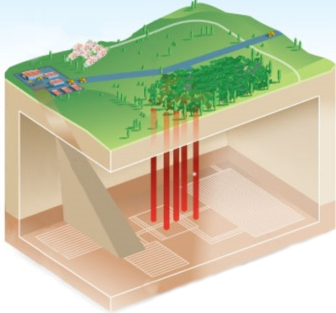
\includegraphics[width=0.75 \textwidth]{stockage_dechets_radioactifs_sans_texte}
% 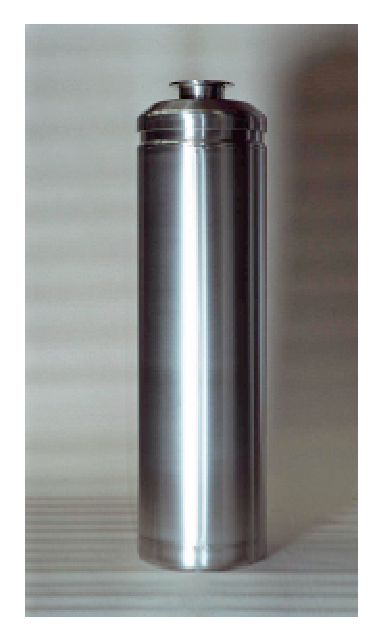
\includegraphics[width = 0.3 \textwidth]{Andra1}
\end{figure}
\end{minipage}
\vspace{-0.05 cm}
\newline
\invisible<2>{
\textcolor{midnightblue}{\textbf{System of
coupled partial differential equations, unsteady problem, strongly nonlinear and degenerate problem, heterogeneous data, phase change:}} \textcolor{red}{\textbf{nonlinear complementarity constraints}}
\\
\vspace*{-0.2 cm}
\invisible<3>{
\begin{center}\textbf{We study 3 problems of increasing difficulty.}
\end{center}
\invisible<4>{
}}}}
\end{frame}
%
\begin{frame}
\frametitle{Motivation}
Consider the system of PDEs with nonlinear complementarity constraints:
\begin{equation*}
\begin{split}
\partial_t \left(\varphi(\bu)\right) + \mathcal{A}(\bu)=\mathcal{F}\\
\textcolor{electricpurple}{\mathcal{K}}(\bu) \geq 0 \quad \textcolor{carmine}{\mathcal{G}}(\bu) \geq 0 \quad \textcolor{electricpurple}{\mathcal{K}}(\bu) \cdot \textcolor{carmine}{\mathcal{G}}(\bu)=0
\end{split}
\end{equation*}
This model is used in various physical phenomena: economy, fluid mechanics, elasticity, multiphase flow.
\\
\textbf{\textcolor{blue}{Numerical resolution:}}

\begin{itemize}
\only<1> {
\item Discretization: Finite elements / finite volumes + backward Euler scheme in time
\begin{equation*}
\begin{split}
\frac{\varphi(\bu_h^n)-\varphi(\bu_h^{n-1})}{t^{n}-t^{n-1}} + \mathcal{A}(\bu_h^{n})=\mathcal{F}_h^{n-1}\\
\textcolor{electricpurple}{\mathcal{K}}(\bu_h^{n}) \geq 0 \quad \textcolor{carmine}{\mathcal{G}}(\bu_h^{n}) \geq 0 \quad \textcolor{electricpurple}{\mathcal{K}}(\bu_h^{n}) \cdot \textcolor{carmine}{\mathcal{G}}(\bu_h^{n})=0
\end{split}
\end{equation*}

\item Nonlinear resolution: semismooth Newton algorithm
\begin{equation*}
\mathbb{A}^{n,\kk-1} \bU_h^{n,\kk} = {\bm F}^{n,\kk-1}
\end{equation*}

}
\only<2> {
\item Discretization: Finite elements /finite volumes + backward Euler scheme in time
\begin{equation*}
\begin{split}
\frac{\varphi(\bu_h^n)-\varphi(\bu_h^{n-1})}{t^{n}-t^{n-1}} + \mathcal{A}(\bu_h^{n})=\mathcal{F}_h^{n-1}\\
\textcolor{electricpurple}{\mathcal{K}}(\bu_h^{n}) \geq 0 \quad \textcolor{carmine}{\mathcal{G}}(\bu_h^{n}) \geq 0 \quad \textcolor{electricpurple}{\mathcal{K}}(\bu_h^{n}) \cdot \textcolor{carmine}{\mathcal{G}}(\bu_h^{n})=0
\end{split}
\end{equation*}

\item  Inexact semismooth Newton algorithm
\begin{equation*}
\mathbb{A}^{n,\kk-1} \bU_h^{n,\kk,\ii} + {\bm R}_h^{n,\kk,\ii} = {\bm F}^{n,\kk-1}
\end{equation*}
}
\end{itemize}
\end{frame}


\begin{frame}
\frametitle{Motivation}
\textbf{\textcolor{blue}{A posteriori error estimate:}} 
\begin{equation*}
\tnorm{\bu-\bu_h^{n,\kk,\ii}} \leq \eta(\bu_h^{n,\kk,\ii}) \quad \mbox{where} \quad \tnorm{\cdot} \quad \mbox{is some norm}
\end{equation*}
\invisible<1>{
\textbf{\textcolor{blue}{Three components of the error:}}
\begin{itemize}
\item discretization error: numerical scheme (finite elements, finite volumes...) ($h,\tau$) \\ 
\item linearization error: semismooth Newton method ($\kk$) \\
\item algebraic error: iterative algebraic solver ($\ii$)
\end{itemize}
\invisible<2>{
\textbf{\textcolor{red}{Questions:}}

Can we distinguish each component of the error? \textcolor{cadmiumgreen}{\textbf{yes!}}
\\
\begin{itemize}
\item $\tnorm{\bu-\bu_h^{n,\kk,\ii}} \leq \eta_{\mathrm{disc}}^{n,\kk,\ii} + \eta_{\mathrm{lin}}^{n,\kk,\ii} + \eta_{\mathrm{alg}}^{n,\kk,\ii}$
\end{itemize}  
\invisible<3>{
Can we reduce the number of iterations? \textcolor{cadmiumgreen}{\textbf{yes!}}
\begin{itemize}
\item Adaptive stopping criterion: semismooth linearization: $\eta_{\mathrm{lin}}^{n,\kk,\ii} \leq \gamma_{\mathrm{lin}} \eta_{\mathrm{disc}}^{n,\kk,\ii}$
\item Adaptive stopping criterion: algebraic: $\eta_{\mathrm{alg}}^{n,\kk,\ii} \leq \gamma_{\mathrm{alg}} \left\{ \eta_{\mathrm{disc}}^{n,\kk,\ii}, \eta_{\mathrm{lin}}^{n,\kk,\ii} \right\}$
\end{itemize}
\invisible<4>{}
}}}
\end{frame}
%
\begin{frame}
\frametitle{Chapter 1: Stationary linear variational inequality}
\vspace{-0.2 cm}
\begin{equation*}
\vspace{-0.2 cm}
\mbox{Find} \quad \bu \in \Kg \quad a(\bu,\bv-\bu) \geq (\bbf,\bv-\bu) \quad \forall \bv \in \Kg
\end{equation*}


\vspace{-0.4 cm}
\begin{figure}
\rotatebox{90}{
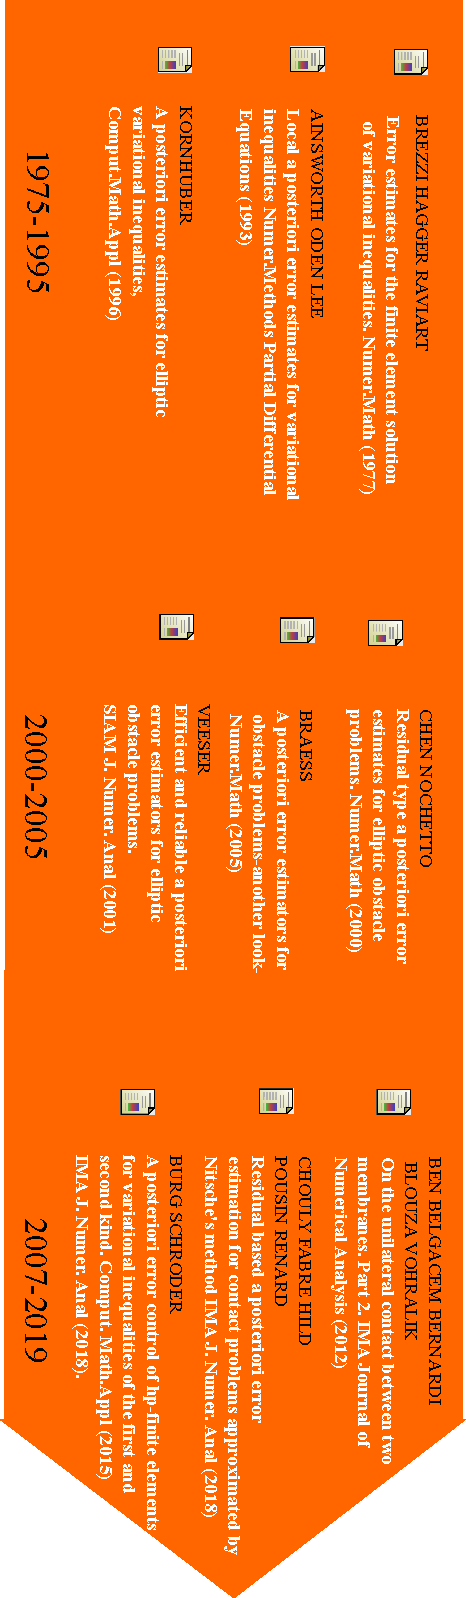
\includegraphics[width = 0.295\textwidth]{Biblio_intro.pdf}}
\end{figure}
\begin{thebibliography}{10}

 \scriptsize{
 \bibitem{Dabaghi:2018}
 {\sc J.~Dabaghi, V.~Martin, and M.~Vohral{\'{\i}}k}, {\em Adaptive inexact
  semismooth Newton methods for the contact problem between two membranes}.
 \textcolor{black}{HAL Preprint~01666845, submitted for publication, 2018}
 }

\end{thebibliography}
\end{frame}
%
\begin{frame}
\frametitle{Chapter 2: Parabolic linear variational inequality}

\begin{equation*}
\mbox{Find} \quad \bu \in \Kgt \quad \langle \partial_t \bu, \bv - \bu \rangle + a(\bu,\bv-\bu) \geq (\bbf,\bv-\bu) \quad \forall \bv \in \Kgt
\end{equation*}
\vspace*{-1 cm}
\begin{figure}
\vspace{0.4 cm}
\rotatebox{90}{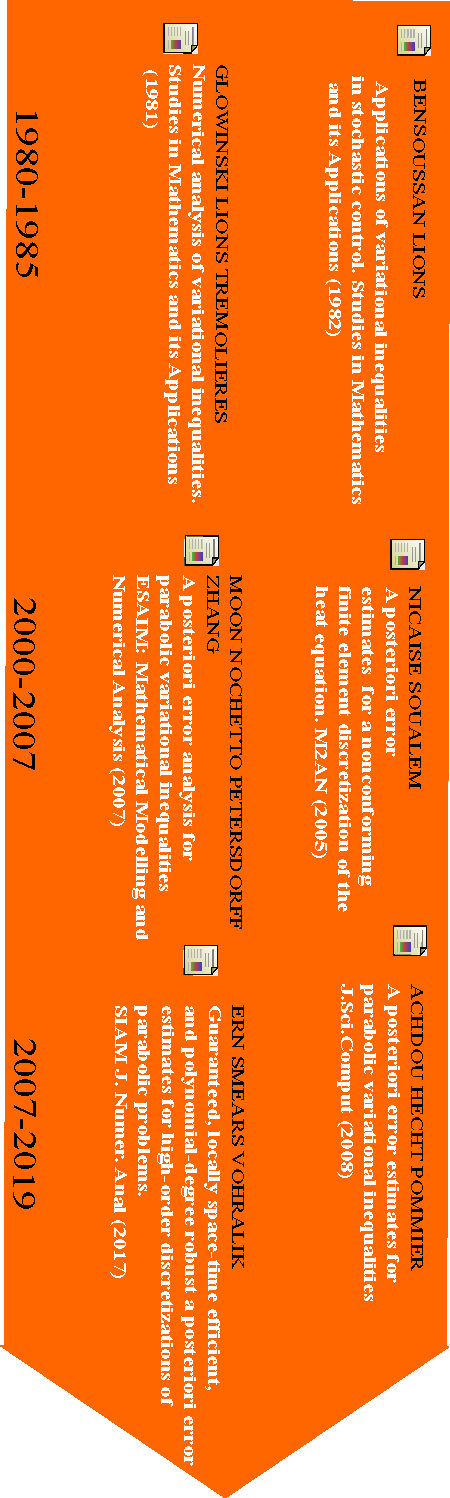
\includegraphics[width = 0.3\textwidth]{Biblio_intro2.pdf}}
\end{figure}


\begin{thebibliography}{10}
 \scriptsize{
 \bibitem{Dabaghi3:2018}
 {\sc J.~Dabaghi, V.~Martin, and M.~Vohral{\'{\i}}k}, {\em A posteriori error estimate and adaptive stopping criteria for a parabolic variational inequality}.
 \textcolor{black}{In preparation, 2019}
 }
\end{thebibliography}

\end{frame}
%
\begin{frame}
\frametitle{Chapter 3: Two-phase compositional flow with phase change}
\vspace{-0.5 cm}
\begin{equation*}
\mbox{Find} \quad \Sl, \Pl, \chihl \quad \dps
\left\lbrace\begin{array}{llccc}
\dps \partial_t l_\componentw(\Sl) + \nab \cdot {\bm \Phi}_{\mathrm{w}}(\Sl,\Pl,\chihl) = Q_{\componentw},  \\
              \dps \partial_t l_\componenth(\Sl,\chihl)  + \nab \cdot {\bm \Phi}_{\mathrm{h}}(\Sl,\Pl,\chihl)=\Qh,\\
\textcolor{electricpurple}{\mathcal{K}}(\Sl) \geq 0, \;  \textcolor{carmine}{\mathcal{G}}(\Sl,\Pl,\chihl) \geq 0, \; \textcolor{electricpurple}{\mathcal{K}}(\Sl) \cdot \textcolor{carmine}{\mathcal{G}}(\Sl,\Pl,\chihl)=0  
\end{array}
\right.
\end{equation*}
\vspace{-0.3 cm}
\begin{figure}
\rotatebox{90}{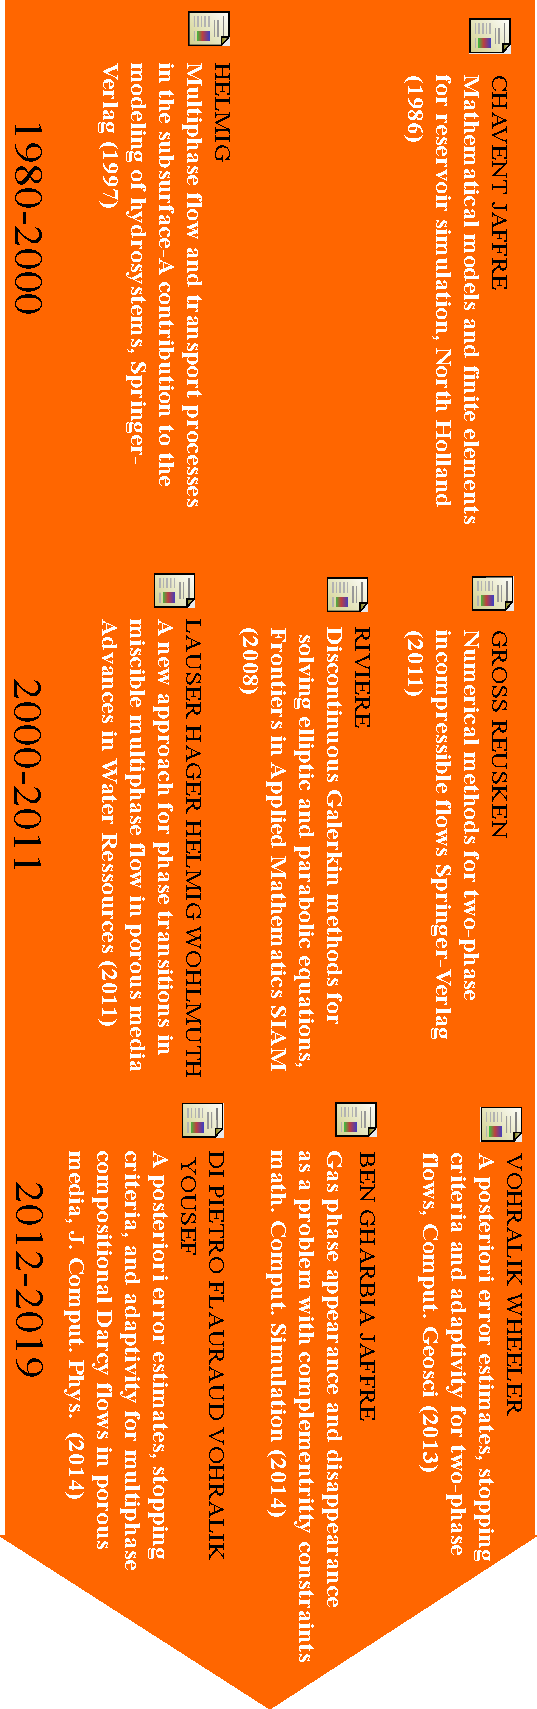
\includegraphics[width = 0.31 \textwidth]{Biblio_intro3.pdf}}
\end{figure}
\vspace{-0.2 cm}
\begin{thebibliography}{10}
 \scriptsize{
 \bibitem{Dabaghi2:2018}
 {\sc I.~Ben Gharbia, J.~Dabaghi, V.~Martin, and M.~Vohral{\'{\i}}k}, {\em A posteriori error estimates and adaptive stopping criteria for a compositional two-phase flow with nonlinear complementarity constraints}.
 \textcolor{black}{HAL Preprint~01919067, In revision, 2019}}
 \end{thebibliography}
\end{frame}
